\documentclass[10pt, letterpaper]{article} % [CHANGED] Mandatory 10pt font and US Letter size
\usepackage{booktabs}

%% Language, font encodings, and Typeface
\usepackage[english]{babel}
\usepackage[utf8x]{inputenc} % Note: utf8 is default in modern LaTeX, but left utf8x to avoid breaking your characters
\usepackage[T1]{fontenc}
\usepackage{mathptmx} % [ADDED] Mandatory Times New Roman typeface

%% Sets page size and margins strictly to ICLR bounds
\usepackage[letterpaper, top=1in, bottom=1in, left=1.5in, right=1.5in, marginparwidth=1.75cm]{geometry} % [CHANGED] Exact dimensions

%% Paragraph formatting
\usepackage{parskip}
\setlength{\parindent}{0pt} % [ADDED] Enforces strict no-indent rule
\setlength{\parskip}{5.5pt plus 1pt minus 1.5pt} % [ADDED] Enforces strict 1/2 line space (11pt leading / 2), with minus glue for vspace squeezing
\usepackage{placeins}

%% Refs pkgs 
\usepackage[style=ieee]{biblatex}
\addbibresource{main.bib}

%% Useful packages
\usepackage{amsmath}
\usepackage{graphicx}
\usepackage{xcolor}
\usepackage[font=small,skip=4pt]{caption} 
\usepackage[colorinlistoftodos]{todonotes}
\usepackage[colorlinks=true, allcolors=blue]{hyperref}
\usepackage{cleveref} 
\usepackage{float}
\usepackage{listings}
\usepackage{diagbox}
\usepackage{multicol}
\usepackage{multirow}

%% [EDIT] VSPACE SAVING HEURISTICS & ICLR HEADING STYLES
\usepackage{titlesec}
% ICLR mandates: 
% Section: 12pt (\large), Small Caps (\scshape), 1 line before, 1/2 line after.
% Subsection: 10pt (\normalsize), Small Caps (\scshape), 1 line before, 1/2 line after.
% *The 'minus' values are our space-saving heuristics—they let LaTeX aggressively squash empty space if the page is getting full.*
\titleformat{\section}{\large\scshape}{\thesection}{1em}{}
\titlespacing*{\section}{0pt}{10pt plus 2pt minus 3pt}{5pt plus 1pt minus 2pt}

\titleformat{\subsection}{\normalsize\scshape}{\thesubsection}{1em}{}
\titlespacing*{\subsection}{0pt}{10pt plus 2pt minus 3pt}{5pt plus 1pt minus 2pt}

\titleformat{\subsubsection}{\normalsize\scshape}{\thesubsubsection}{1em}{}
\titlespacing*{\subsubsection}{0pt}{8pt plus 2pt minus 2pt}{4pt plus 1pt minus 1pt}

% Squeeze space around floats (figures/tables)
\setlength{\textfloatsep}{8pt plus 2pt minus 4pt}
\setlength{\floatsep}{4pt plus 1pt minus 2pt}
\setlength{\intextsep}{8pt plus 2pt minus 4pt}
\setlength{\dbltextfloatsep}{8pt plus 2pt minus 4pt}
\setlength{\dblfloatsep}{6pt plus 2pt minus 2pt}

% Squeeze space around math equations
\setlength{\abovedisplayskip}{4pt plus 1pt minus 2pt}
\setlength{\belowdisplayskip}{4pt plus 1pt minus 2pt}
\setlength{\abovedisplayshortskip}{2pt plus 1pt minus 1pt}
\setlength{\belowdisplayshortskip}{2pt plus 1pt minus 1pt}
%% [/EDIT]

\lstset{
  basicstyle=\ttfamily,
  columns=fullflexible,
  frame=single,
  breaklines=true,
  postbreak=\mbox{\textcolor{red}{$\hookrightarrow$}\space},
  showstringspaces=false
}
\AtBeginBibliography{\footnotesize}

\begin{document}

%% [EDIT] Better title blurb with University of Southampton and fixed \hline
\begin{center}
    {\LARGE \scshape CoTFormer Reproducibility Report} \\[1em]
    {\normalsize \textbf{Alberto Berni} (ab3u21)\textsuperscript{1}, \textbf{Bryan Vullo} (bv1g22)\textsuperscript{1}, \textbf{Tevfik Aras Kavuncu} (tak1e25)\textsuperscript{1}} \\[0.2em]
    {\normalsize \textsuperscript{1}\textit{University of Southampton, School of Electronics and Computer Science}}
\end{center}
\vspace{-0.5em}

\setlength{\parskip}{0.1cm}
\setlength{\parindent}{0cm}

\section{Introduction}\label{sec:intro}
% Setting
%   - Transformer      -v                                   (1)
%   - Parallel compute -> Paran inefficiency                (2)
%   - What led to BUT - recurrent inductive bias        
% CoT                                                       (3)
%   - CoT Paper
% BUT                                                       (4)
%   - Recurrent
%   - better param efficiency - overwrite representations
%   - released before CoT
% What makes CoTFormer interesting                          (5)
%   - Solves representations loss
%   - intermediate representation
%   - more representations

% The Transformer architecture has become the dominant backbone for language modelling, largely by replacing recurrent computation with parallel self-attention \cite{vaswani2017attention}. This design has proved highly scalable, but it also raises a long-standing question in neural algorithmic reasoning: whether purely feed-forward depth provides the right inductive bias for computations that are naturally iterative. Earlier work on Neural GPUs showed that recurrent parameter sharing can support algorithmic generalization from short training instances to longer test instances \cite{kaiser2016neural}. Universal Transformers later reintroduced recurrence into self-attention by repeatedly applying the same Transformer block, combining global attention with a recurrent computational structure \cite{dehghani2019universal}. 

% This issue has become newly relevant in the context of chain-of-thought reasoning. Chain-of-thought prompting improves performance by allowing a model to generate intermediate reasoning steps before producing a final answer \cite{wei2022chain}. CoTFormer builds on this observation by arguing that chain-of-thought resembles repeatedly applying a Transformer, while also preserving a crucial distinction: generated intermediate states can attend to previous intermediate states, unlike in standard weight-tied recurrence \cite{mohtashami2025cotformer}. This motivates architectures that bake latent recurrent computation into the model rather than relying only on explicit natural-language reasoning traces.

% However, evaluating such architectures only through language-modelling perplexity may obscure the behaviour they are designed to improve. Recent work on looped Transformers argues that ``perplexity, although very useful for training, is a narrow measure of model quality'', and shows that looped models can exhibit better reasoning behaviour despite worse perplexity and memorization than iso-FLOP non-looped baselines \cite{saunshi2025reasoning}. In particular, Saunshi et al. report that looped models disproportionately improve reasoning-heavy tasks, and that middle-looping---keeping the first and last layers independent while looping only the middle block---can be a more practical variant than looping the entire model \cite{saunshi2025reasoning}. This is closely aligned with CoTFormer's reserved-layer design, where beginning and final layers are separated from the repeated middle computation block.

% In this work, we evaluate whether this recurrent inductive bias helps on a controlled algorithmic generalization task. We focus on shifted-start inductive counting, a setting designed to prevent trivial position-based solutions and to test whether models can extrapolate beyond the cardinalities observed during training \cite{chang2025counting}. We compare a standard Transformer, a Block Universal Transformer, and a fixed-depth CoTFormer with separated repeated middle layers. This allows us to ask whether CoTFormer's CoT-like latent recurrence provides benefits beyond both ordinary feed-forward depth and standard weight-tied looping.
Transformers replaced recurrence with parallel self-attention, enabling scalable language modelling but weakening the architectural bias toward iterative computation \cite{vaswani2017attention}. This tension is central to neural algorithmic reasoning: earlier recurrent models (i.e. Neural GPUs) could generalise from short training instances to longer algorithmic inputs through repeated parameter sharing \cite{kaiser2016neural}, and Block Universal Transformers (BUT) later reintroduced this idea by repeatedly applying the same Transformer block \cite{dehghani2019universal}. 
%% COULD REMOVE
% Wei et al. discovered the same recurrent principle as an emergent capability of language models: attending to intermediate reasoning tokens improves model performance on difficult reasoning tasks \cite{wei2022chain}. 

The CoTFormer architecture formalises this connection by treating Chain-of-thought as a form of \emph{recurrent latent computation}. CoTFormer preserves previous intermediate states as attendable representations, more closely mimicking how explicit thought tokens can attend to earlier thought tokens \cite{cotformer}. Authors evaluate this architecture through perplexity and compute efficiency, despite recent related work suggesting that ``\emph{perplexity, although very useful for training, is a narrow measure of model quality}'', showing looped models can improve reasoning-heavy tasks despite worse perplexity and memorisation than iso-FLOP non-looped baselines \cite{saunshi2025reasoning}. This motivates evaluating CoTFormer not only as a language model, but as a recurrent architecture with a potential inductive bias for iterative reasoning. We reproduce and evaluate the main claims of CoTFormer and its variants, and extend its evaluation to ask \emph{whether its recurrent structure improves controlled algorithmic generalisation}.
% Methodology
% 1. How did we train (L4s, Batch sizes, gradient acc, RNG state restoration)
% 2. Other technical items we say "we mention them when relevant"
\section{Methodology}\label{sec:methodology}

Reproduction of this work\footnote{Recorded on \href{https://github.com/COMP6258-Reproducibility-Challenge/CoTFormer}{GitHub}, forked from the \href{https://github.com/epfml/CoTFormer}{original}.} was performed on L4 GPUs, requiring specific adaptations to the original codebase, designed for A100 GPUs. To reconcile this divergence, we applied the following:

\textbf{Minor Adaptations} Reduced vRAM budget required lowering batch size and proportionally increasing gradient accumulation steps, retaining the original batch size (128). Evaluation of MAC metrics was estimated in closed-form due to these constraints. 

\textbf{LN-CoTFormer} We initially trained this variant to 40k steps for \Cref{tab:table2-repro}, resuming to 60k steps for further evaluation. This invalidated the previous learning-rate scheduler, requiring use of a different one and causing the 0.4 perplexity divergence observed in \Cref{tab:section5-pair}.

\textbf{ADM Distributed Training} The original repository bypassed RNG state check-pointing (required by the ADM). 
Replacing the NCCL backend with Gloo guaranteed RNG state restoration while confounding training dynamics (\cref{sec:ADM}). For other experiments a seperate branch fixed NCCL's deadlock and RNG state checkpointing issues.
% NCCL was replaced with Gloo as a replacement during the reproduction of some models. Whilst NCCL's deadlock issue was fixed later on for later reproduction.

\section{Reproduction}
% Experiments
% 1) Table 1
%   - Base CoTFormer
%   - results with delta
%   - SEM (Std err mean)
%   - Match claims?
%   - interesting results... TBD
%   - Data/train split (HFX)

% 2) Figs 2 & 3
%   - results
%   - match claims?
%   - interesting - TBD on graphs

% 3) Table 2
%   - results
%   - match claims?
%   - interesting:
%     - 2 -> 21x5 -> 1 (Res. only)
%       - phase change
%       - Aras' diagnostics
%     - No KV cache
%     ? LNCoT:
%       - track layer-norm weights!
%   - Why layer norm?
%   - LNCoT (40k)
%     - outperforms BUT baseline x48
%     - claim validated
\paragraph{Base CotFormer} 
Base CoTFormer models are reproducible; we notice ``\emph{benign spikes}'' during training, later explored in~\cref{subsec:phase-change}.
% The Figures 1a, 1b, and 2 \autoref{fig:2ab-and-3} 
\begin{figure}[H]
    \centering
    % --- Image (a) ---
    \begin{minipage}{0.27\textwidth}
        \centering
        \textbf{\scriptsize(a)} \\
        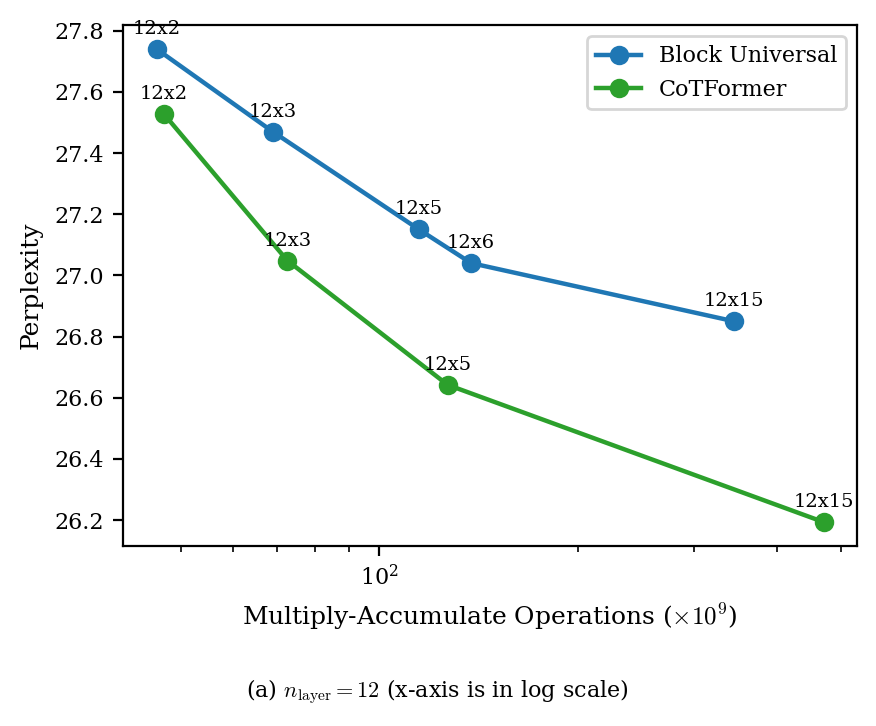
\includegraphics[width=\linewidth]{img/fig2a.png}
    \end{minipage}% <--- The % kills the invisible space
    \hspace{1em}
    % --- Image (b) ---
    \begin{minipage}{0.27\textwidth}
        \centering
        \textbf{\scriptsize(b)} \\
        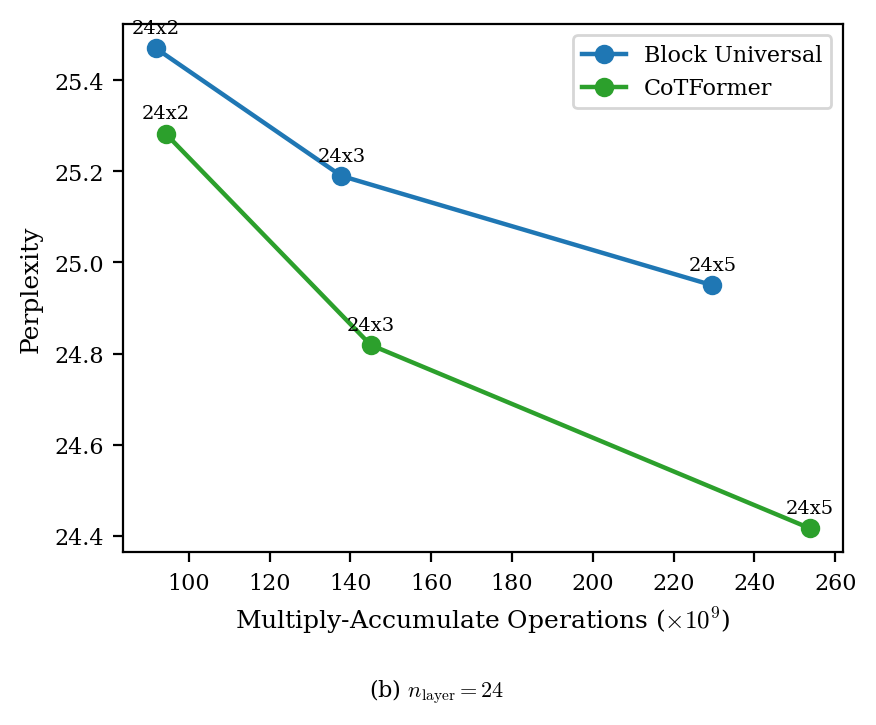
\includegraphics[width=\linewidth]{img/fig2b.png}
    \end{minipage}%
    \hspace{1em}
    % --- Image (c) ---
    \begin{minipage}{0.27\textwidth}
        \centering
        \textbf{\scriptsize(c)} \\
        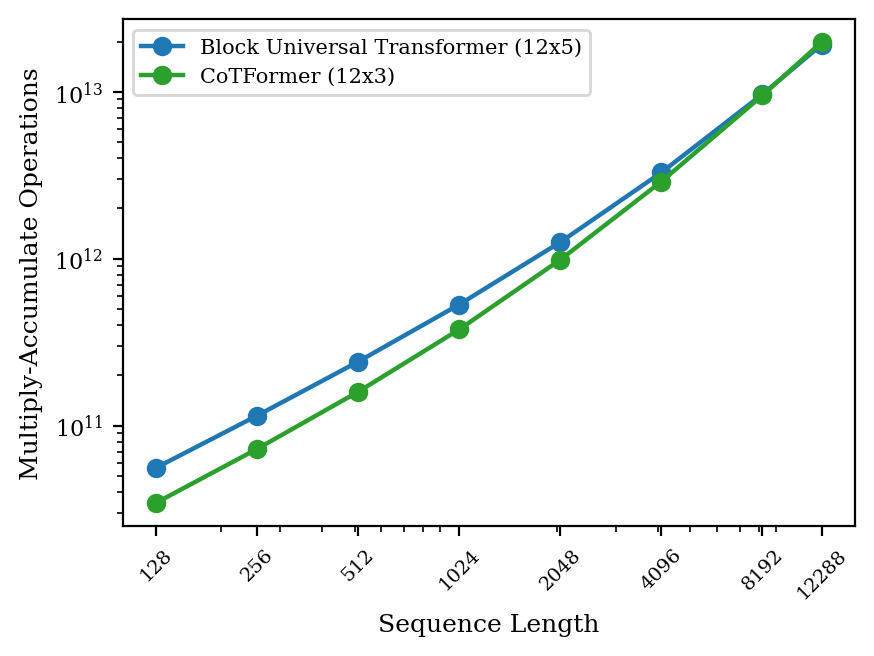
\includegraphics[width=\linewidth]{img/fig3.png}
    \end{minipage}%
    \caption{\centering\textbf{(a)-(b)} Reproduced comparison of BUT (original results) and CotFormer pareto curves; \textbf{(c)} Reproduced comparison of compute intensity when performance is comparable. (Paper fig. 1a, 1b, 2)}
    \label{fig:2ab-and-3}
\end{figure}
\FloatBarrier
\begin{table}[ht]
\centering
\resizebox{\textwidth}{!}{%
\begin{tabular}{lc|ccc|ccc|ccc}
\toprule
 & & \multicolumn{3}{c|}{Theirs} & \multicolumn{3}{c|}{Ours} & \multicolumn{3}{c}{$\Delta$ (Ours $-$ Theirs)} \\
\multirow{2}{*}{Model} & \multirow{2}{*}{Base Layers ($n_\text{layer}$)} & \multicolumn{3}{c|}{$n_\text{repeat}$} & \multicolumn{3}{c|}{$n_\text{repeat}$} & \multicolumn{3}{c}{$n_\text{repeat}$} \\
\cmidrule(lr){3-5} \cmidrule(lr){6-8} \cmidrule(lr){9-11}
 & & 2 & 3 & 5 & 2 & 3 & 5 & 2 & 3 & 5 \\
\midrule
CoTFormer                   & 12 & \textbf{27.55 (0.02)} & \textbf{27.07 (0.01)} & \textbf{26.64 (0.04)} & \textbf{27.53 (0.67)} & \textbf{27.05 (0.65)} & \textbf{{26.64 (0.64)}} & $-0.02$ & $-0.02$ &{$0.00$} \\
\midrule
CoTFormer                   & 24 & \textbf{25.28 (0.00)} & \textbf{24.85 (0.04)} & \textbf{24.48 (0.03)} & \textbf{25.28 (0.61)} & \textbf{24.82 (0.59)} & \textbf{24.42 (0.58)} & $\phantom{-}0.00$ & $-0.03$ & $-0.06$ \\
\bottomrule
\end{tabular}%
}
\caption{Perplexity comparison. \emph{Theirs}: SEM over 3 seeds (paper Table~1). \emph{Ours}: single seed; uncertainty is per-batch CI$_{95}$. $\Delta$ shows the difference in perplexity (Ours $-$ Theirs); negative values means our run is better.}
\label{tab:table1}
\end{table}
\paragraph{CoTFormer Variants} The original CoTFormer architecture is extended by three compounding variants: \textbf{i.}~a standard CoTFormer that reserves first and last layers for embedding translation alone \textbf{ii.}~LN-CoTFormer adds a post-repeat LayerNorm to stabilise the recursive residual stream, and \textbf{iii.}~Adaptive Depth Module (ADM) to dynamically route token computation and reduce recurrence during inference. We reproduce the variants below and evaluate their structural hypotheses.
% TODO: Update 25x5 CoTFormer Results when ready
\begin{table}[H]
\centering
\resizebox{\textwidth}{!}{%
\begin{tabular}{llcccc}
\toprule
\textbf{Variant} & \textbf{Layers (effective)} & \textbf{Paper PPL (SEM)} & \textbf{Ours PPL (SEM)} & $\Delta$ & \textbf{95\% CI (ours)} \\ \midrule
CoTFormer & $24\times5\qquad\qquad\;\;(120)$ & 24.48 (0.03) & 24.42 & $-0.06$ & [23.84, 25.01] \\
CoTFormer + Reserved & 24, 2$\rightarrow$21$\times$5$\rightarrow$1 (108) & 24.51 (0.01) & 24.64 & +0.13 & [24.25, 25.03] \\
LN-CoTFormer ($40$k)& 24, 2$\rightarrow$21$\times$5$\rightarrow$1 (108) & 24.11 (0.03) & 24.13 & +0.02 & [23.75, 24.51] \\ \bottomrule
\end{tabular}%
}
\caption{Reproduction of the CoTFormer's Table 2 results at \texttt{40k} training steps.}
\label{tab:table2-repro}
\end{table}
\paragraph{Reserved Layers \& LN-CoTFormer}\label{sec:RLLN}
CoTFormer with Reserved Layers reproduces its original results within statistical bounds (\Cref{tab:table2-repro}). This change alone\footnote{Isolating recurrent reasoning in a central block by reserving the first and last layers strictly for embedding translation.} \emph{isn't} more parameter-efficient than the baseline Transformer (48L) nor the CoTFormer ($24\times5$) on perplexity alone . The 24-layer model effectively executes a 108-layer forward pass, showing it can \emph{approximate} deeper standard model capacity, paying a cost in sheer performance. \textbf{LayerNorm:} Authors justify this variant claiming ``\emph{it is important to maintain a consistent input’s scale (across repeats)}''; the insight follows from the original architecture's \cite{vaswani2017attention} and remains empirically valid given the 0.51 PPL improvement from the baseline CoTFomer. Crucially, the variant outperforms the 48-layer Transformer baseline, a much more widely adopted architecture, by 0.29 PPL. While the result shows recursive computation (similarly to parallel counterparts) benefits from explicit feature scaling to prevent representation drift, it fails to explain \emph{why} this is the case.

\paragraph{ADM CoTFormer}\label{sec:ADM} By employing a ``\emph{Mixture of Repeats}'' strategy with randomized capacities, the ADM trains a routing mechanism to decide whether a token requires further recurrent processing~\cite{cotformer}. While the original Figure 4 (\cref{fig:adm-evaluation}\textbf{(a)}) can be replicated, the core claim that ``\emph{the ADM can efficiently route computation based on token difficulty}'' cannot be confirmed as it lacks a clear definition of efficiency: showing the ADM outperforms its fixed-compute-budget copy is hardly a proof of this. 
\begin{figure}[H]
    \centering
    % --- Image (a) ---
    \begin{minipage}{0.23\textwidth}
        \centering
        \textbf{\scriptsize(a)} \\
        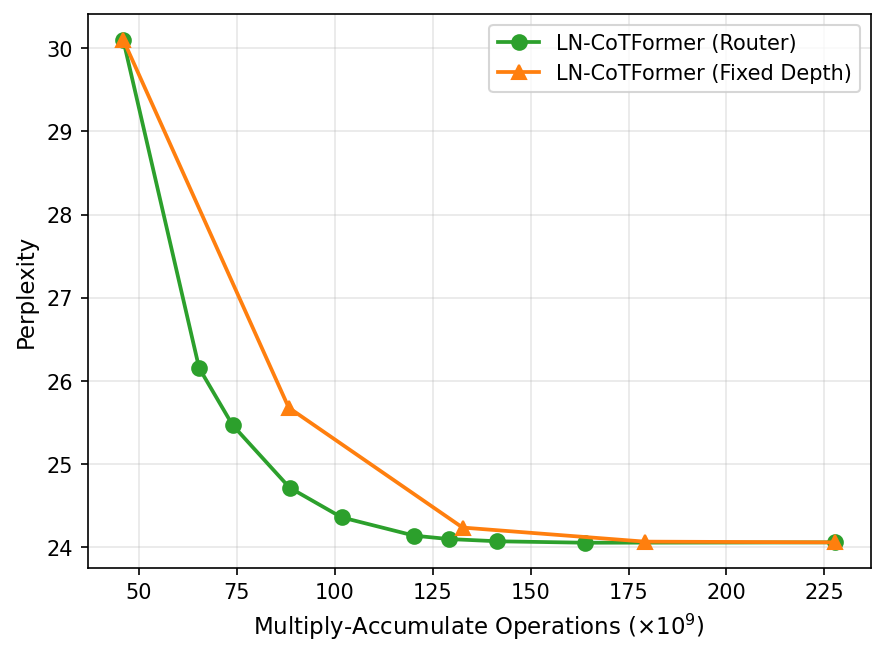
\includegraphics[width=\linewidth]{img/figure4_pareto.png}
    \end{minipage}% <--- The % kills the invisible space
    \hfill
    % --- Image (b) ---
    \begin{minipage}{0.23\textwidth}
        \centering
        \textbf{\scriptsize(b)} \\
        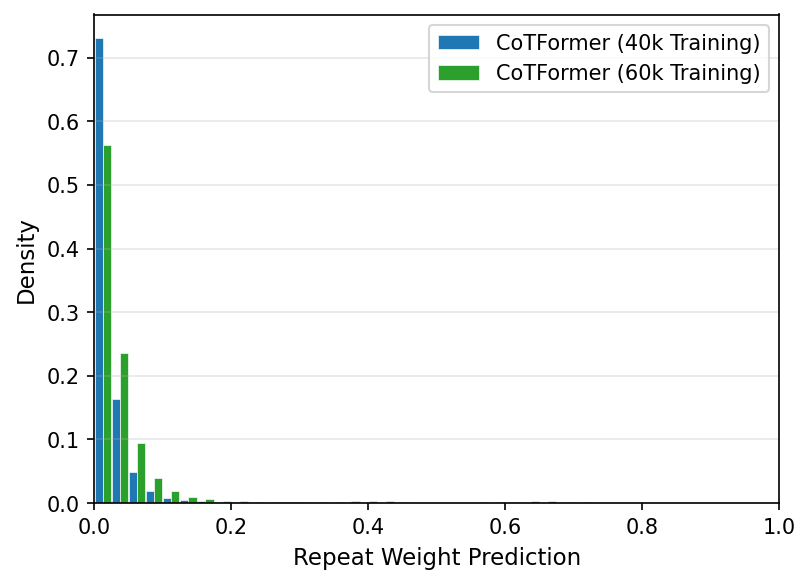
\includegraphics[width=\linewidth]{img/figure5_raw.png}
    \end{minipage}%
    \hfill
    % --- Image (c) ---
    \begin{minipage}{0.23\textwidth}
        \centering
        \textbf{\scriptsize(c)} \\
        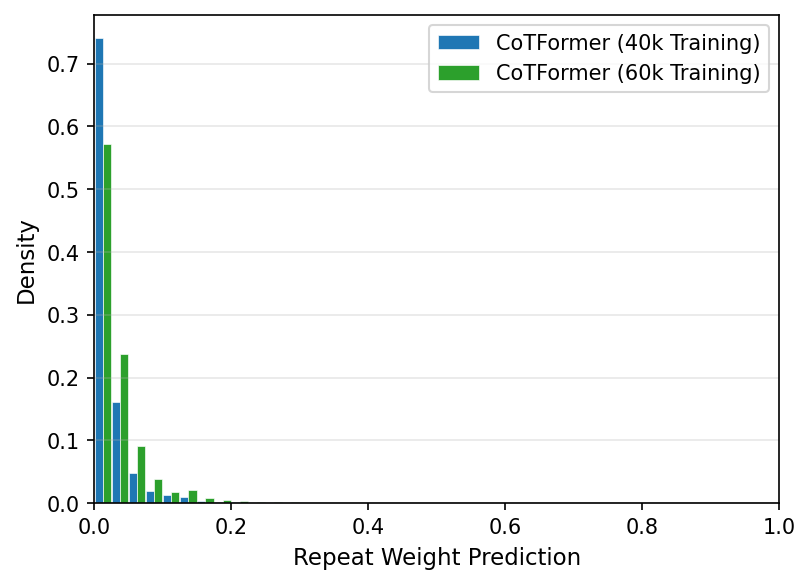
\includegraphics[width=\linewidth]{img/figure5_picascade.png}
    \end{minipage}%
    \hfill
    % --- Image (d) ---
    \begin{minipage}{0.23\textwidth}
        \centering
        \textbf{\scriptsize(d)} \\
        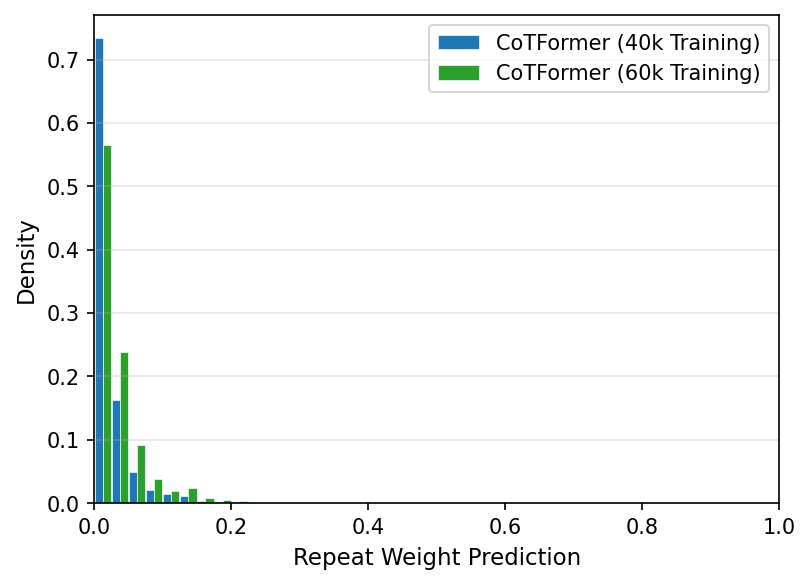
\includegraphics[width=\linewidth]{img/figure5_ptcascade.png}
    \end{minipage}
    \caption{\centering\textbf{(a)} Reproduced Pareto curve of compute vs perplexity; \textbf{(b)-(d)} Comparison of router weight extraction methods (raw, per-index cascade, and per-token cascade) at 40k and 60k training steps.}
    \label{fig:adm-evaluation}
\end{figure}
\vspace{-1em}
 \paragraph{Irreproducible claims} Authors state the adaptive model ``\emph{would benefit more from longer training}'', proposing extended training budgets. Using Figure \cite{cotformer}, they argue the model ``\emph{increasingly utilises deeper repeats over time}''. The claims are unrelated: increased usage of final repeats only proves the model allocates more compute; verifying a predictive benefit requires controlled evaluation at matched inference compute (i.e. \cref{fig:2ab-and-3}). Further, the authors' extraction script contains an inaccuracy in how it orders extracted weights (\texttt{get\_router\_weights.py}, 129-131), whereby the intended ``\emph{final repeat}'' becomes a cascaded minimum across repeats. We replicate this exactly in \cref{fig:adm-evaluation}~\textbf{(c)}, further evaluating two different extraction methods (\cref{fig:adm-evaluation}): \textbf{(b)}~the raw router weights, and \textbf{(d)}~corrected per-token cascade. Across all histograms, densities decay drastically compared to the original figure: ADM final repeat usage is lower than claimed. This divergence is confounded by back-end divergences; we can qualitatively confirm a \emph{marginal} increase in final repeat usage in longer training, but cannot conclude whether the claimed distribution is genuine or a by-product of our constraints.
\begin{table}[H]
\centering
\resizebox{0.6\textwidth}{!}{%
\begin{tabular}{lccc}
\toprule
\textbf{Model} & \textbf{Paper PPL} & \textbf{Ours PPL (SEM)} & $\Delta$ \\ \midrule
LN CoTFormer 60k & 23.19 & 23.59 (0.01) & +0.40 \\
ADM 60k (full compute) & 23.83 & 24.06 (0.01) & +0.23 \\ \midrule
Adaptive cost & +0.64 & +0.47 & N/A \\ \bottomrule
\end{tabular}%
}
\caption{\centering Reproduced CoTFormer Section 5 PPL\cite{cotformer} comparison at 60k training steps.}
\label{tab:section5-pair}
\end{table}

\section{Extensions}
% \paragraph{Training Stability} We did not observe the ``\emph{benign spikes}'' in gradient norms reported by the authors. Gradients remained stable (0.49--0.54) across models' training steps, hinting this might be an artifact of original training hardware or (consequently) larger batch sizes with lower gradient accumulation.
\subsection{Phase change analysis} \label{subsec:phase-change}
We notice a significant shift in attention distribution across CoTFormer repeat states during training (\cref{fig:combined-cascade-plots}). Around 27k training steps, attention mass redistributes rapidly across different repeat budgets, accompanied by ``\emph{benign spikes}'' in gradient norm and a substantial increase in within-repeat attention entropy for certain repeats. We interpret this as \emph{faint} evidence of repeat-state specialisation: middle blocks may learn non-uniform uses of latent repeat states. Establishing if these correspond to algorithmic recurrent reasoning requires additional experiments, which we leave to future work.
\begin{figure}[H]
    \centering
    \begin{minipage}{0.18\textwidth}
        \centering
        \textbf{\scriptsize(a)}\\
        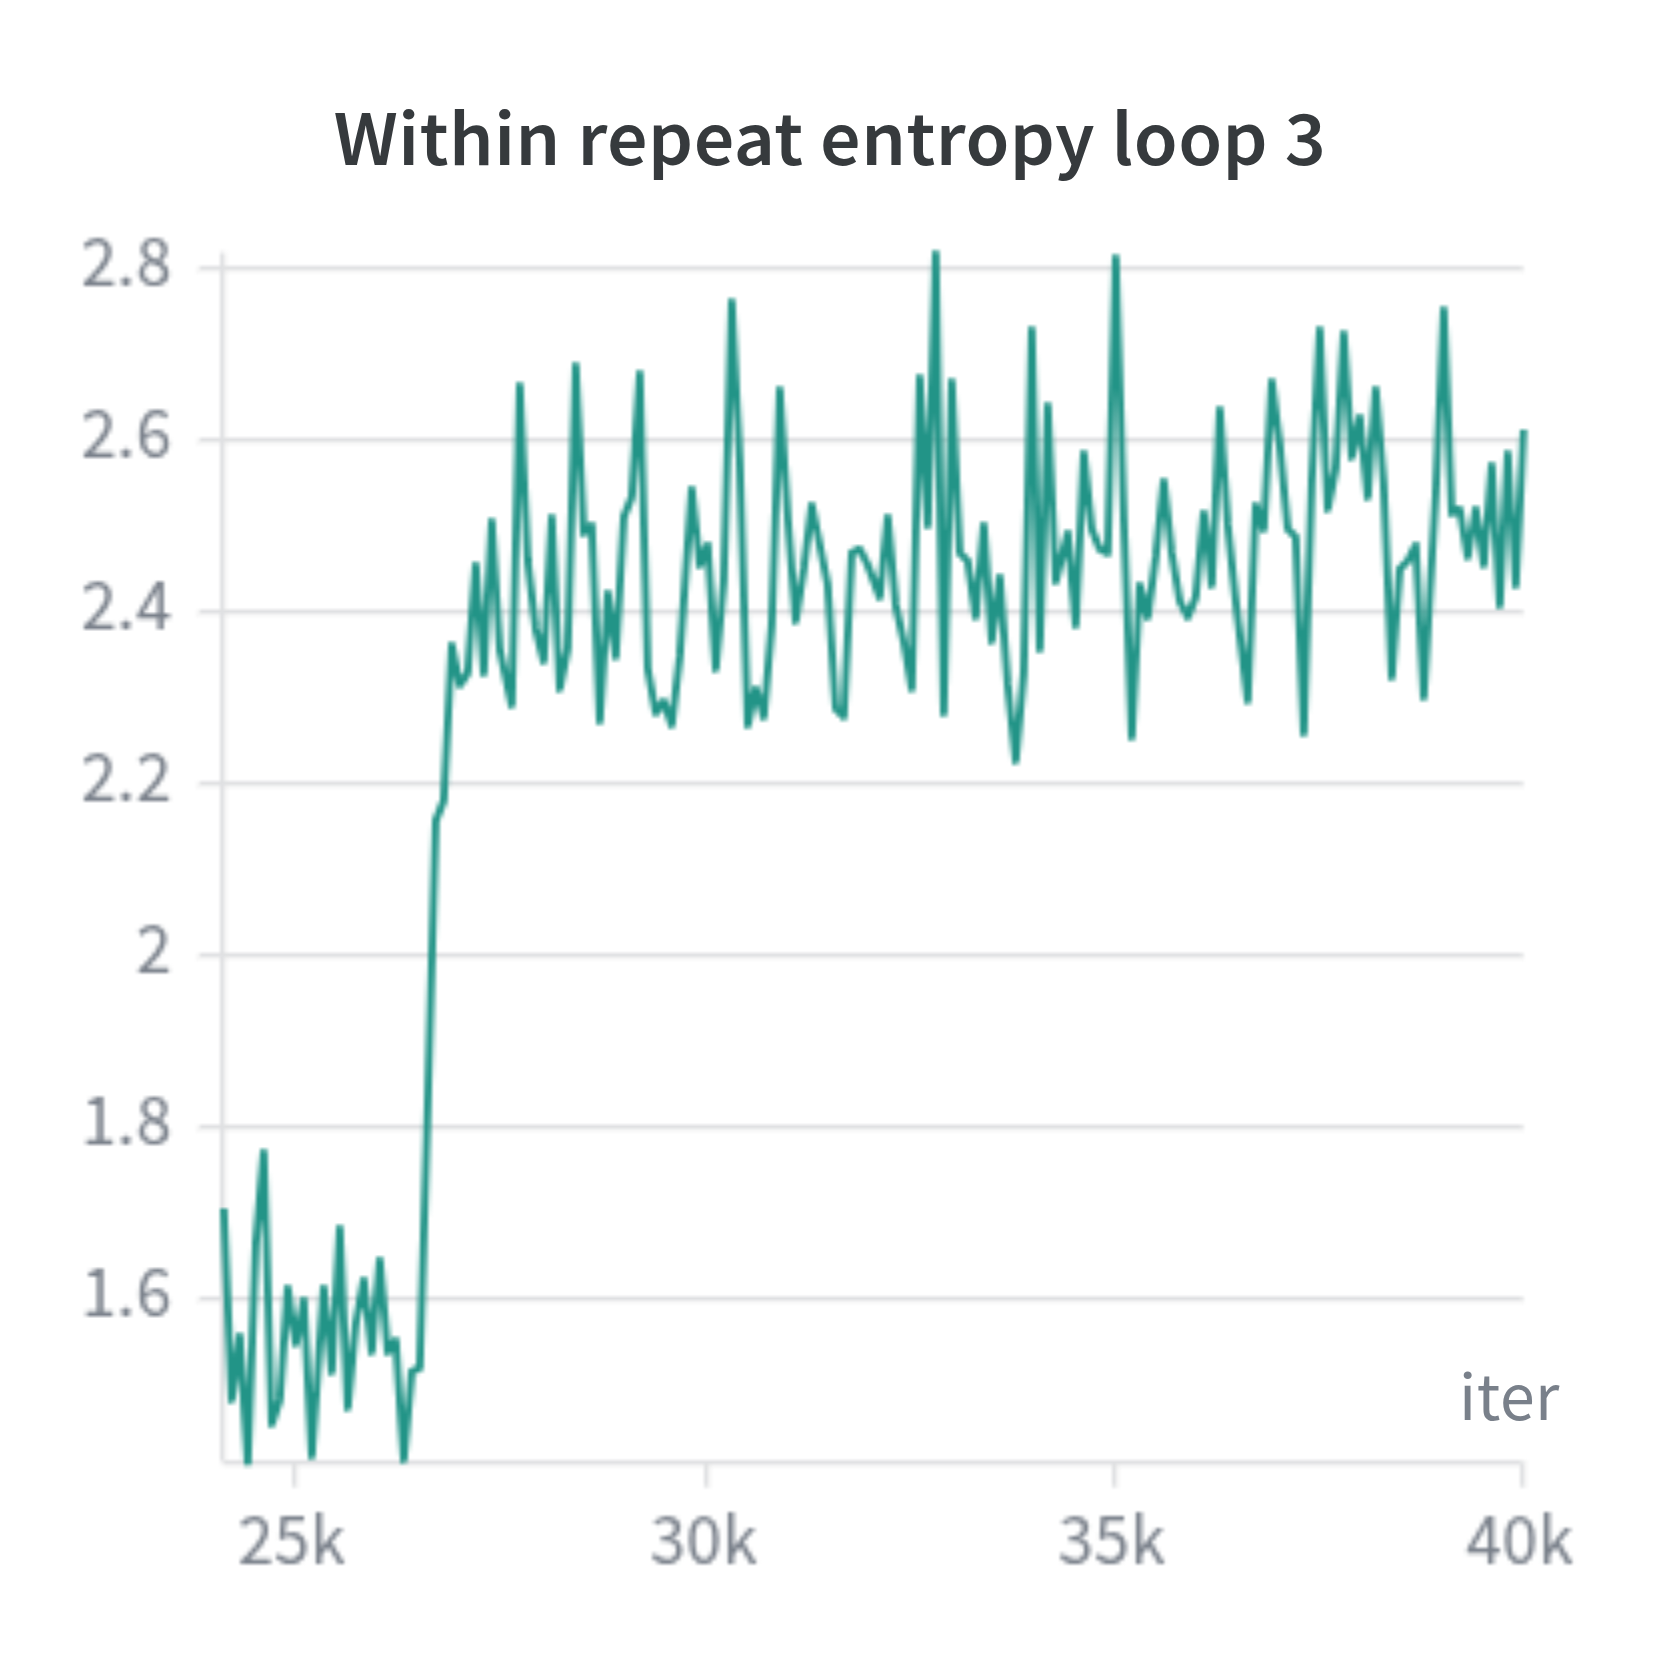
\includegraphics[width=\textwidth]{img/within_Rep_loop_3.png}
    \end{minipage}
    \hspace{1em}
    \begin{minipage}{0.18\textwidth}
        \centering
        \textbf{\scriptsize(b)}\\
        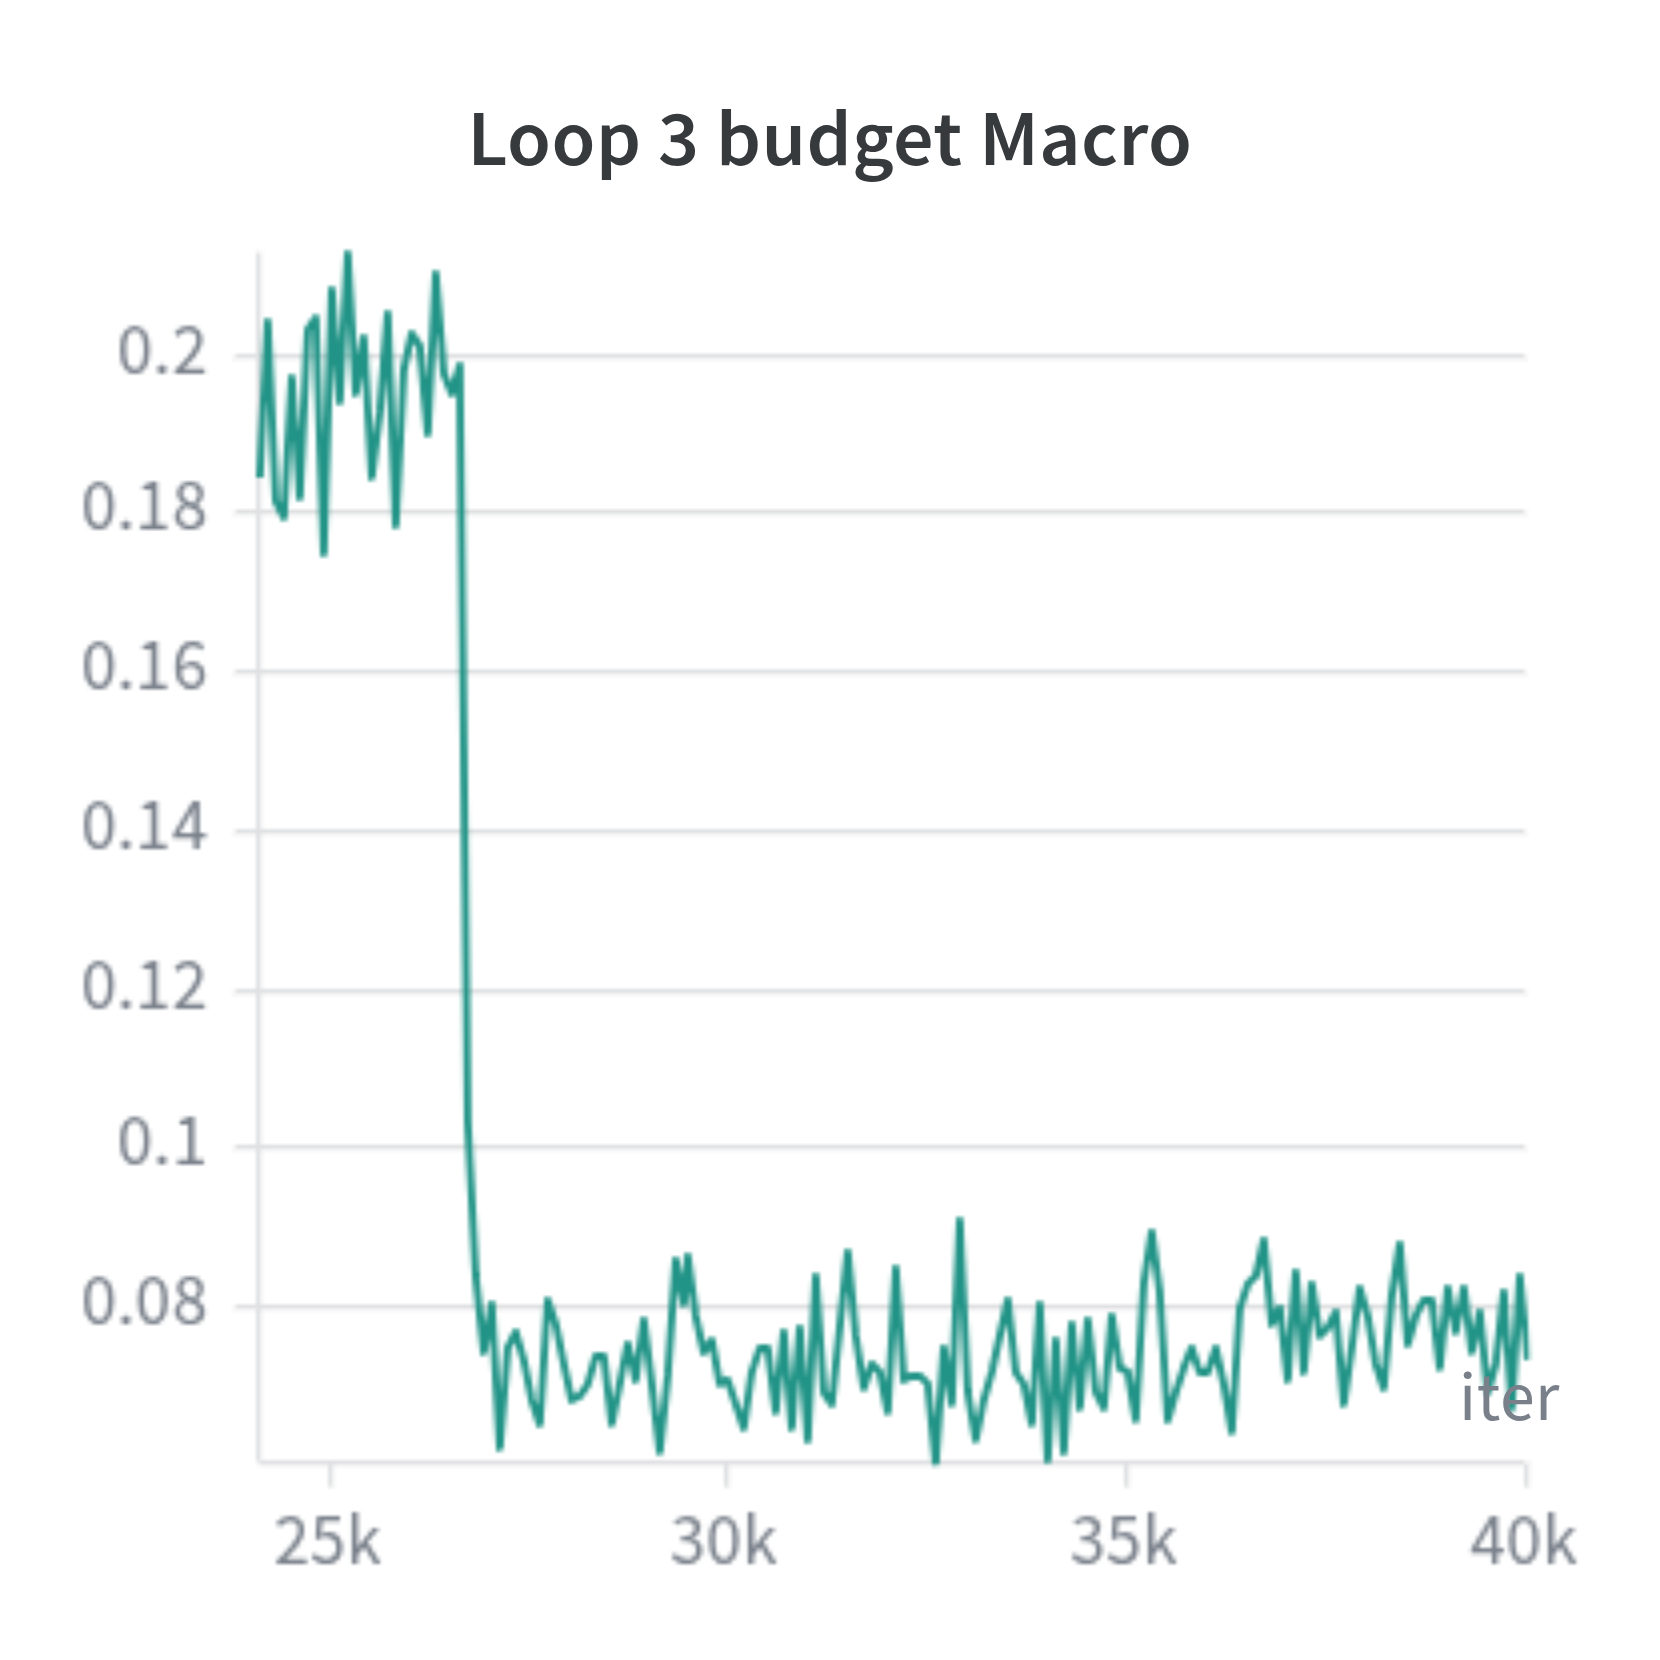
\includegraphics[width=\textwidth]{img/macro_l3.png}
    \end{minipage}
    \hspace{1em}
    \begin{minipage}{0.18\textwidth}
        \centering
        \textbf{\scriptsize(c)}\\
        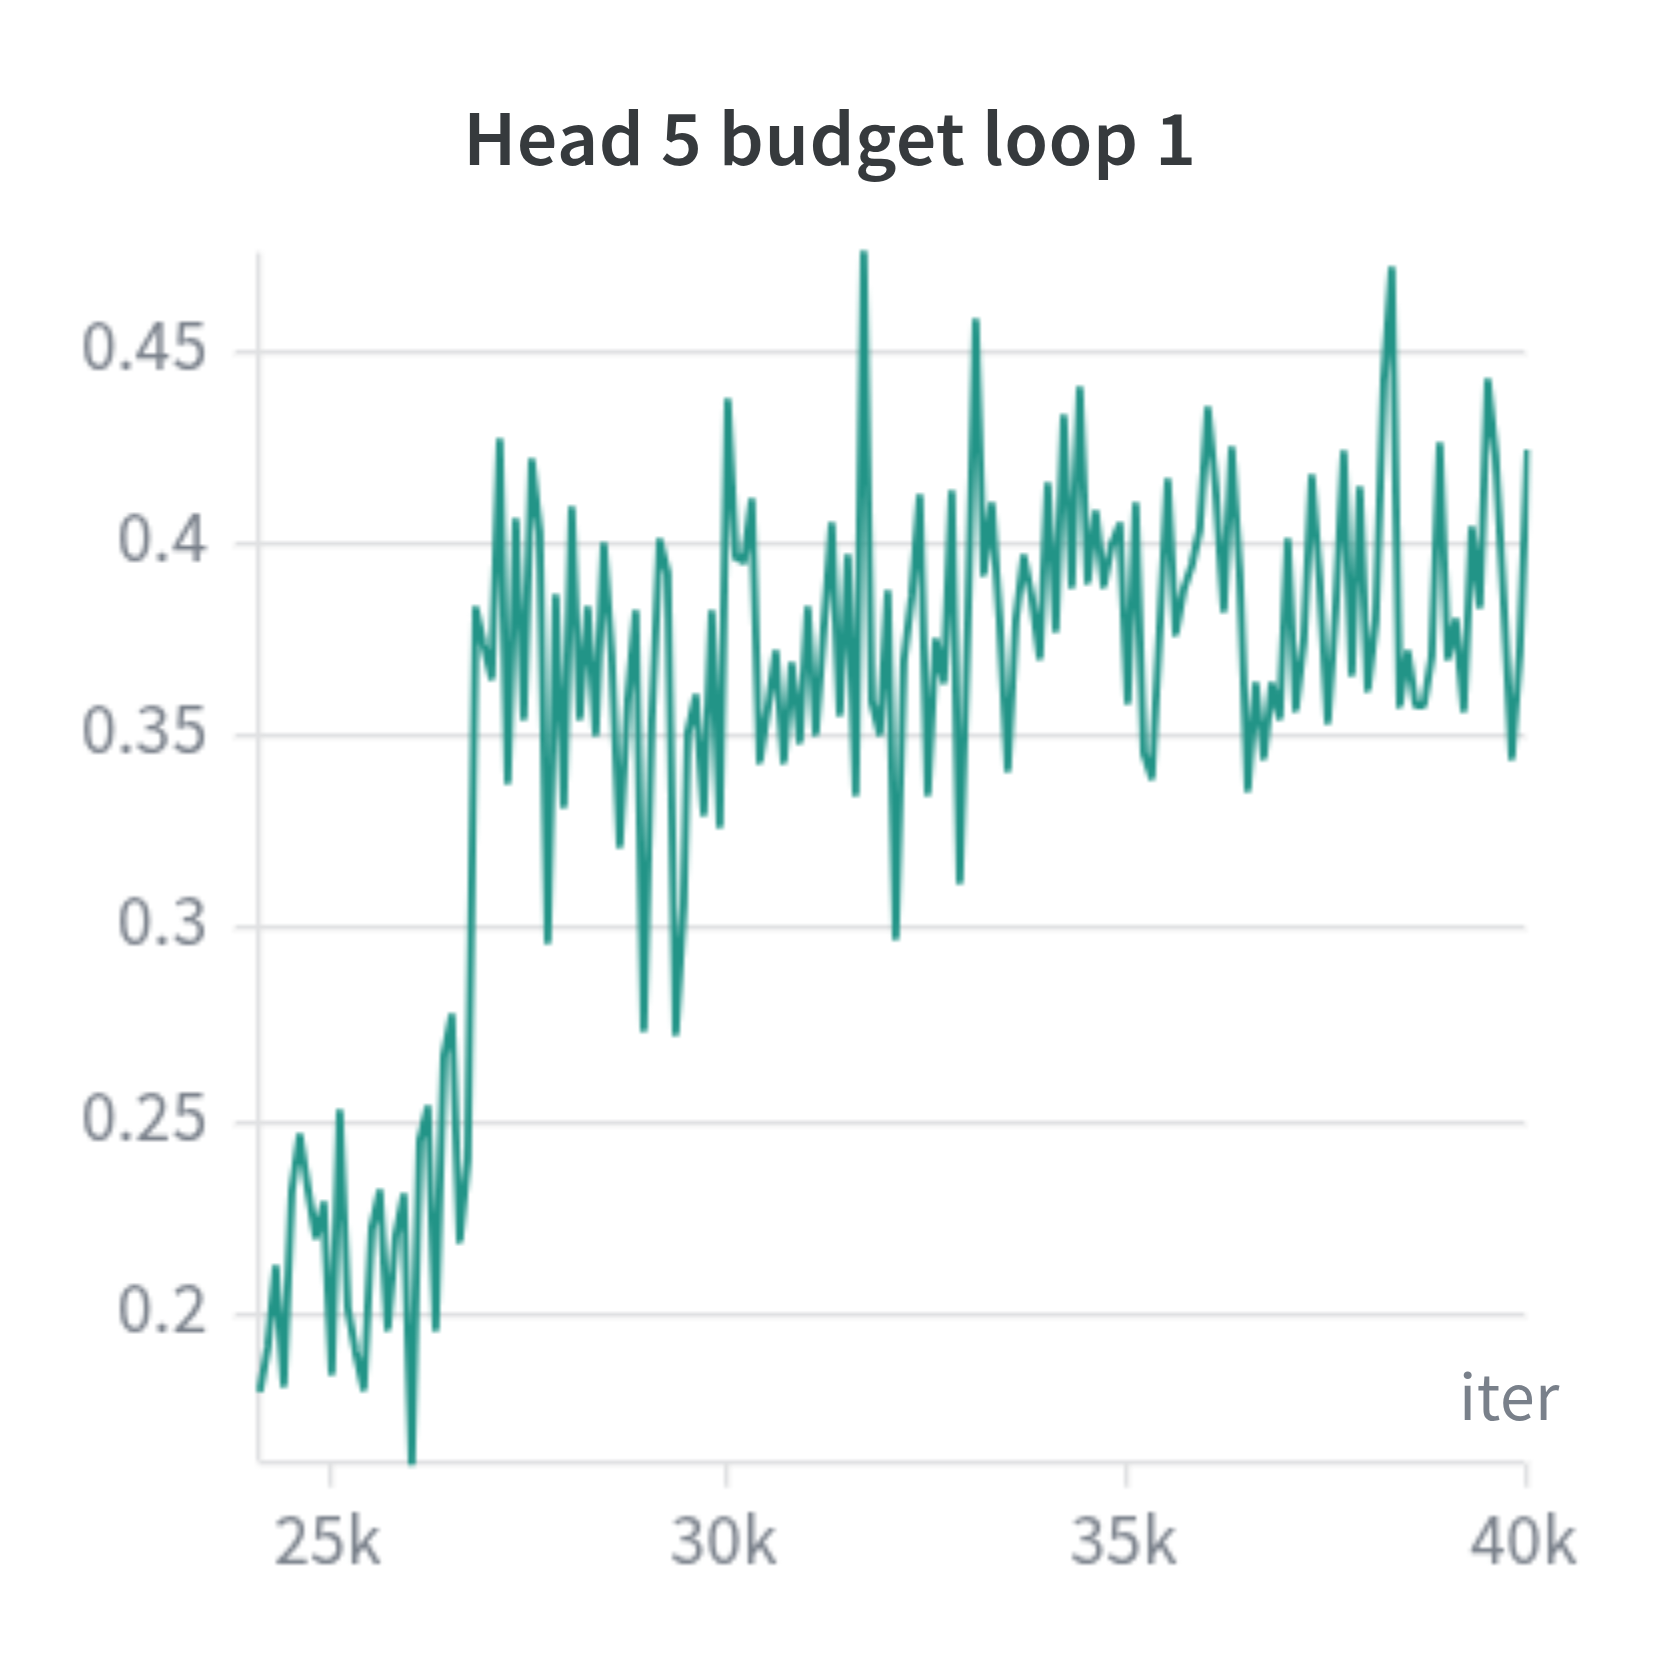
\includegraphics[width=\textwidth]{img/head_5_budget_loop1.png}
    \end{minipage}
    \hspace{1em}
    \begin{minipage}{0.18\textwidth}
        \centering
        \textbf{\scriptsize(d)}\\
        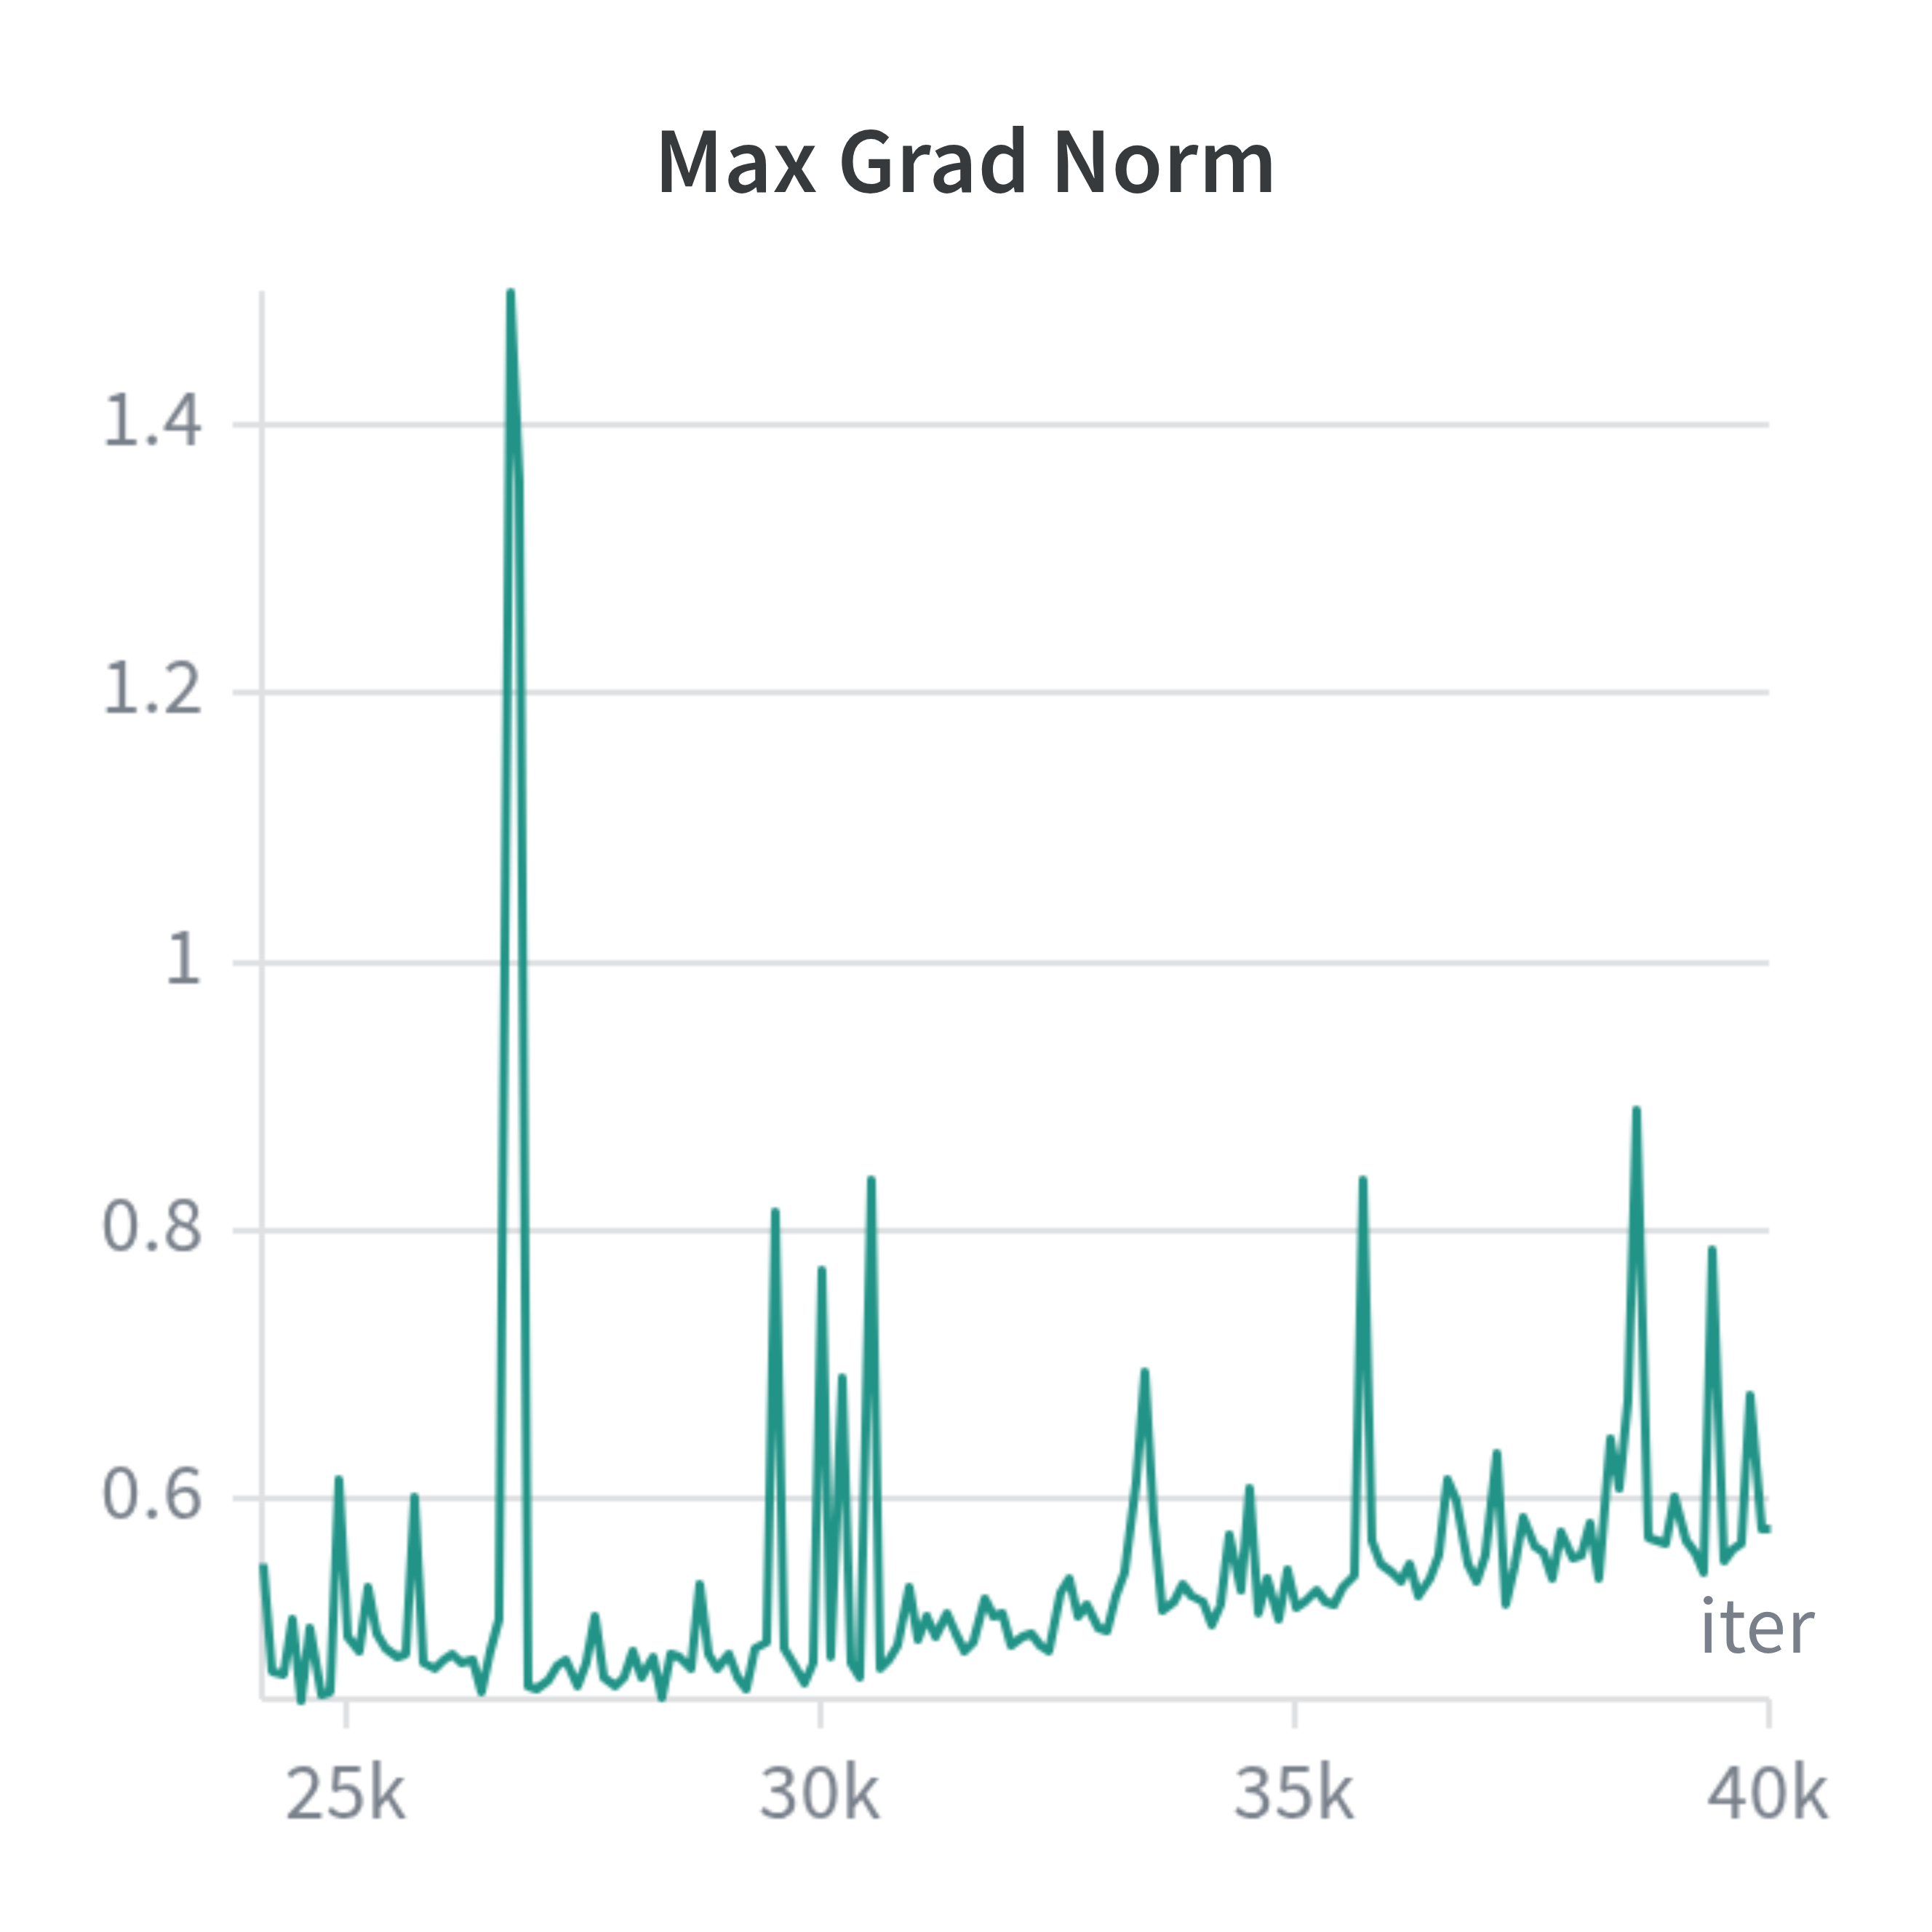
\includegraphics[width=\textwidth]{img/max_grad_norm.png}
    \end{minipage}

    \caption{Repeat-state attention reorganisation during OWT2 training of a 2→24×5→1 CoTFormer.}
    \label{fig:combined-cascade-plots}
\end{figure}
% Theory: Phase changes
%   - "Within-loop entropy"
%   - look at how model attends to shift
%   - around 27k steps
%   - No LN full depth
%   - Could be like LN-CoT "benign spikes" we don't know
%   - Yes, there's some form of CoT happening
% Experiment: Inductive bias "Counting"
%   - genenrate monotonic int seqs
%   - train model
%   - Can it count? OOD?
%   - Shifted start?
%   - Modular counting???

% > we'll shorten these as well --aras


\subsection{Shifted Start and P-hop}
To answer our research question (\cref{sec:intro}) we adapt the shifted-start counting task from Chang and Bisk~\cite{chang2025counting}, extending the limited training split with variable-length examples below the maximum training length. Early high-width runs were unstable and prone to overfitting, so we reduced width to 128 and used 4 heads while keeping the expanded dataset. Across BUT, CoTFormer and Transformer baselines, OOD accuracy remained capped around 0.26--0.27. Increasing loop depth did not improve extrapolation under teacher-forced sequence prediction, suggesting that models may rely on \emph{positional shortcuts} rather than an iterative counting procedure. The strongest single-seed result came from the reserved-layer CoTFormer, although the effect is seed-sensitive.

\begin{table}[H]
\centering
% \caption{Shifted-start OOD accuracy.}
\label{tab:ood_acc_summary}
{\small
\renewcommand{\arraystretch}{0.78}
\setlength{\tabcolsep}{4pt}
\setlength{\aboverulesep}{0.25ex}
\setlength{\belowrulesep}{0.25ex}
\setlength{\heavyrulewidth}{0.08em}
\setlength{\lightrulewidth}{0.04em}
\begin{tabular}{lrrrr}

\toprule
Model & Seeds & Mean OOD acc & Std & Max OOD acc \\
\midrule
CoTFormer: \(1 \to 1{\times}3 \to 1\) & 4 & \textbf{0.267977} & 0.009061 & \textbf{0.280910} \\
CoTFormer: \(1{\times}8\)             & 2 & 0.259697 & 0.003039 & 0.261846 \\
CoTFormer: \(1{\times}4\)             & 4 & 0.261681 & 0.003881 & 0.266346 \\
Base: \(4{\times}1\)                  & 4 & 0.267383 & 0.002967 & 0.270341 \\
Base: \(1{\times}1\)                  & 4 & 0.234779 & 0.003352 & 0.238078 \\
\bottomrule
\end{tabular}
}
\caption{Shifted-start OOD accuracy.}
\end{table}

\begin{table}[H]
\centering

\label{tab:phop_results}
{\small
\renewcommand{\arraystretch}{0.85}
\setlength{\tabcolsep}{4pt}
\begin{tabular}{lrrrr}
\toprule
Model & Eff. depth & Step & Val acc & Test acc \\
\midrule
Base Transformer \(1{\times}1\)        & 1 & 240k & 0.4659 & 0.4676 \\
Base Transformer \(6{\times}1\)        & 6 & 300k & 0.6121 & 0.6133 \\
CoTFormer \(1{\times}4\)               & 4 & 248k & 0.5935 & 0.6005 \\
BUT \(1{\times}6\)                     & 6 & 250k & 0.6582 & 0.6597 \\
CoTFormer \(1{\times}6\)               & 6 & 300k & \textbf{0.6627} & \textbf{0.6619} \\
CoTFormer \(1 \to 1{\times}4 \to 1\)   & 6 & 272k & 0.6605 & 0.6585 \\
\bottomrule
\end{tabular}
}
\caption{Single-seed p-hop induction results on constructive \(p=32\), \(n=256\), \(|\Sigma|=4\).}
\end{table}

Unlike shifted-start inductive counting, the p-hop task benefits from repeated computation. In shifted-start counting, increasing loop depth did not improve OOD extrapolation suggesting that recurrence over layers did not induce a true counter-like procedure, while on p-hop induction, looped models clearly outperform shallow Transformer baselines on this run. The \(1{\times}1\) Transformer reaches only \(0.4676\) test accuracy, while \(1{\times}6\) BUT and CoTFormer reach roughly \(0.66\). This supports a task-dependent interpretation: looped computation appears useful when the target algorithm resembles repeated retrieval or pointer chasing, but it does not automatically provide the successor-state mechanism required for inductive counting.

The CoTFormer-specific advantage is modest. CoTFormer \(1{\times}6\) slightly outperforms BUT, and the reserved-middle variant \(1 \to 1{\times}4 \to 1\) performs similarly. These results support the usefulness of repeated latent computation for p-hop induction, but do not isolate a large benefit of CoTFormer's cache mechanism over vanilla block looping. 


\section{Conclusion}
We largely reproduce the main CoTFormer perplexity results, including the benefit of post-repeat LayerNorm, but find the adaptive-depth claims less clean: ADM preserves a compute--perplexity tradeoff, while its reported deep-repeat usage is sensitive to extraction method and training confounders. Our extensions suggest a narrower interpretation of CoTFormer’s recurrent bias. Repeated latent computation helps on p-hop induction, where the target resembles iterative retrieval, but does not by itself induce robust OOD counting on shifted-start. Thus, CoTFormer appears promising as a compute-sharing architecture with task-dependent algorithmic benefits, rather than a general mechanism for latent chain-of-thought reasoning. Stronger claims require matched-compute evaluations, more seeds, and controlled tasks isolating when recurrence learns an actual iterative procedure.

\printbibliography[heading=bibnumbered, title={References}]
\end{document}
\printbibliography[heading=bibnumbered, title={References}]
\end{document}